\chapter{Einleitung}
Dieses Dokument dient der genaueren Beschreibung und Dokumentation des Entwurfs zum Visualisierungstool \gls{programname}, dessen Hauptaufgabe die Darstellung des Netzwerkverkehrs eines \gls{profinet}-Systems ist. Des Weiteren wird der im \gls{ids} \gls{snort} eingebaute \gls{praeprozessor} \gls{sppname} und die genaue Funktionsweise der \gls{ipc} zu \gls{programname} erläutert.\newline
 \newline
Der Entwurf von \gls{programname} baut auf das klassische \gls{mvc} Design auf, welches bereits im Pflichtenheft präsentiert wurde. Abbildung~\ref{fig:arch_diagram} zeigt den erweiterten Aufbau des \gls{mvp} Musters. Im Folgenden wird auf die einzelnen Komponenten dieses Diagramms genauer eingegangen.\newline
\begin{figure}[H]
  \centering
  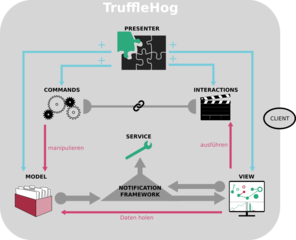
\includegraphics[width=0.8\textwidth]{../diagramimages/arch_diagram_mvp_test.png}
  \caption[Erweiterte Architekturübersicht]{Erweiterte Architekturübersicht}
  \medskip
  Erweiterte Strukturierung des Programms nach dem \gls{mvp} Muster
  \label{fig:arch_diagram}
\end{figure}\newpage

\textbf{MODEL:}\newline
Wie im traditionellen \gls{mvc} Muster dient das Model ausschließlich zur Speicherung von Daten in geeigneten Datenstrukturen. Im Fall von \gls{programname} umfasst dies den Graphen (Kapitel~\ref{subsubsec:graph}), die Programmeinstellungen (Kapitel~\ref{subsubsec:configdata}), Filter (Kapitel~\ref{subsubsec:filter}) und das Graphdatenlog (Kapitel~\ref{subsubsec:graphlog}). \newline
 \newline
\textbf{VIEW:}\newline
Auch der View unterscheidet sich kaum von der ursprünglichen Funktionalität. Er dient weiterhin dazu, dem Benutzer eine Plattform zur Interaktion mit dem Programm zu bieten. Ein wesentlicher Unterschied zum ursprünglichen Aufbau ist hierbei jedoch, dass der View nur spezifische Interaktionen (siehe Kapitel~\ref{subsec:interaction}: interaction) kennt und ausführen kann. Wobei der View keine Kenntnis über die hinter der Aktion stehende Logik hat. \newline
 \newline
\textbf{INTERACTIONS:}\newline
Wie bereits im vorherigen Absatz beschrieben, dienen Interaktionen dem View als Verknüpfung zwischen den tatsächlich ausgeführten Commmands und den Nutzerinteraktionen.\newline
 \newline
\textbf{COMMANDS:}\newline
Commands enthalten neben dem service Package den Großteil der Programmlogik und werden von den entsprechenden Services ausgeführt.\newline
 \newline
\textbf{PRESENTER:}\newline
Der Presenter leistet die gesamte Aufbauarbeit. Commands werden mit bestimmten Interaktionen verknüpft, grafische Oberflächen werden instanziiert und vorbereitet und das Modell wird erstellt.
Zusätzlich kümmert sich der Presenter darum, dass sämtliche Service Routinen gestartet werden und dass das Notification Framework initialisiert wird.\newline
 \newline
\textbf{SERVICE:}\newline
Die Bestandteile des service Packages sind eigenständige Programmroutinen. Entkoppelt von dem Rest des Programms erledigen sie Aufgaben und kommunizieren mittels des Notification Frameworks mit anderen Teilnehmern des Programms.\newline
 \newline
\textbf{NOTIFICATION FRAMEWORK:}\newline
Das Notification Framework dient zur Kommunkation zwischen den einzelnen Programmteilen, wobei diese voneinander entkoppelt bleiben.
